\documentclass[superscriptaddress,aps,prb,11pt]{revtex4-1}

\usepackage{amsmath}
\usepackage{graphicx}
\usepackage{color}
\usepackage{subfigure}
\usepackage{hyperref}

\begin{document}

\title{Experimental Search for Lorentz Violation in Antihydrogen}
\author{F. Isono}
\affiliation{Department of Physics, University of California, Berkeley, CA 94720-7300, USA}
\affiliation{Department of Energy Sciences, Tokyo Institute of Technology, Yokohama, 226-8502, Japan}

\author{Z. Vendeiro}
\affiliation{Department of Physics, University of California, Berkeley, CA 94720-7300, USA}

\author{J. Fajans}
\affiliation{Department of Physics, University of California, Berkeley, CA 94720-7300, USA}
\affiliation{Lawrence Berkeley National Laboratory, Berkeley, CA 94720, USA}

\author{A. Charman}
\affiliation{Department of Physics, University of California, Berkeley, CA 94720-7300, USA}
\affiliation{Lawrence Berkeley National Laboratory, Berkeley, CA 94720, USA}

\author{M. Reinsch}
\affiliation{Department of Physics, University of California, Berkeley, CA 94720-7300, USA}
\affiliation{Lawrence Berkeley National Laboratory, Berkeley, CA 94720, USA}

\author{J. S. Wurtele}
\affiliation{Department of Physics, University of California, Berkeley, CA 94720-7300, USA}
\affiliation{Lawrence Berkeley National Laboratory, Berkeley, CA 94720, USA}

\author{A. Lotta-Folks}
\affiliation{Department of Physics, University of California, Berkeley, CA 94720-7300, USA}
\affiliation{Lawrence Berkeley National Laboratory, Berkeley, CA 94720, USA}

\begin{abstract}
Data on locations of antihydrogen annihilations in the ALPHA trap is retrospectively analyzed for temporal variation due to violations of Lorentz Invariance as the Earth rotates and orbits the sun.  To be continued\ldots
\end{abstract}

\maketitle

\section{Introduction}
General relativity purports that a particle's charge is independent of the observer's reference frame.  Although the theoretical underpinnings of this prediction are strong, experimental verification of fundamental predictions of physics are critical to assessing the axioms necessary to develop such theory.  In this spirit, we have performed a retrospective analysis on the data collected during the ALPHA experiment's runs in 2010 and 2011 to examine it for indications of Lorentz violation in the antimatter sector.

Proposed violations are expected to be correlated with the velocity and/or orientation of the trap relative to a preferred frame.  As is common in searches for Lorentz violation, speed is measured relative to the rest frame of the CMB.  The Earth's CMB speed varies by $\sim\!\!15\%$ as it orbits the sun (see Fig \ref{fig:true_event_distribution}).

\begin{figure}
  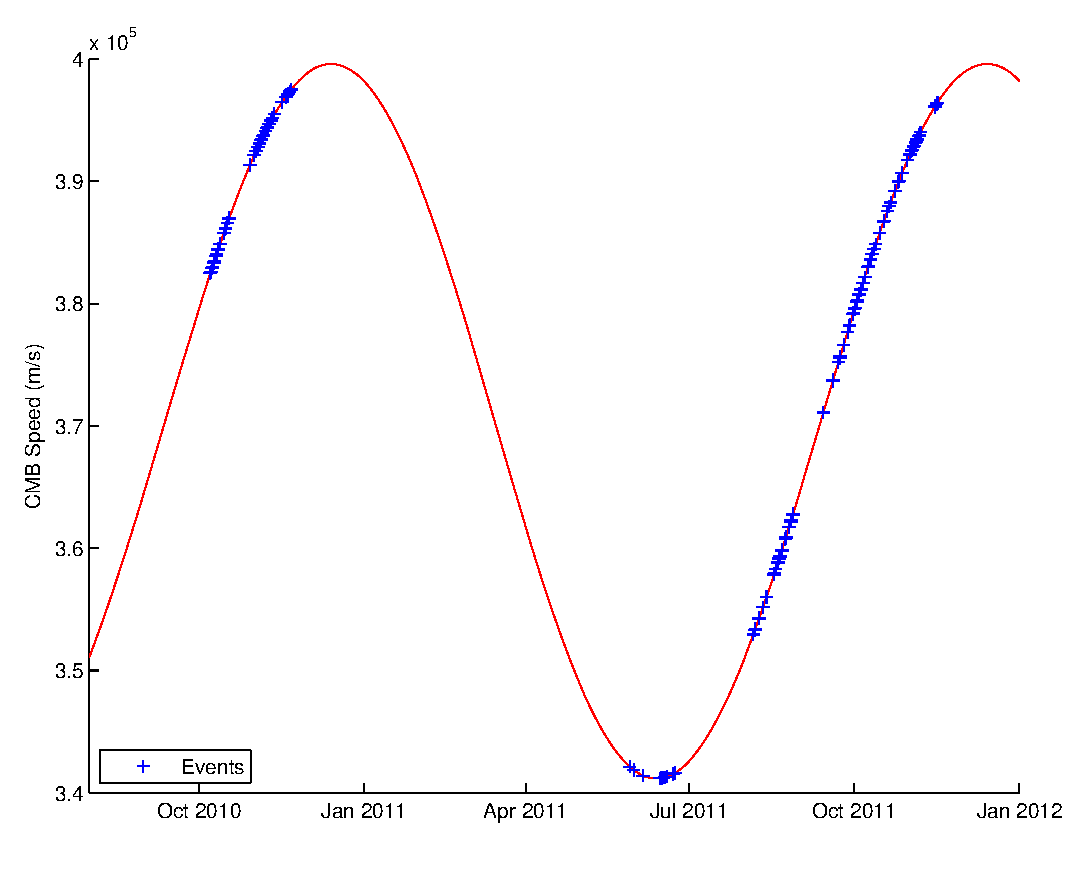
\includegraphics[scale=0.5]{True_Event_Distribution.eps}
  \caption{The CMB speed of the Earth over the period of time during which ALPHA was running.  Times of the $\bar{H}$ annihilation events are marked.}
  \label{fig:true_event_distribution}
\end{figure}

Over 386 antihydrogens in 320 experimental runs passed all detection criteria, hereafter referred to as cuts\cite{amol:14a}.  Only the antihydrogens that passed the cuts are included in the analysis.  The times of these events were distributed over 405 days and over all hours of the day, (see Fig.\ref{fig:eventTime_date_experiment}), which covers both annual and daily cycles.

\begin{figure}
  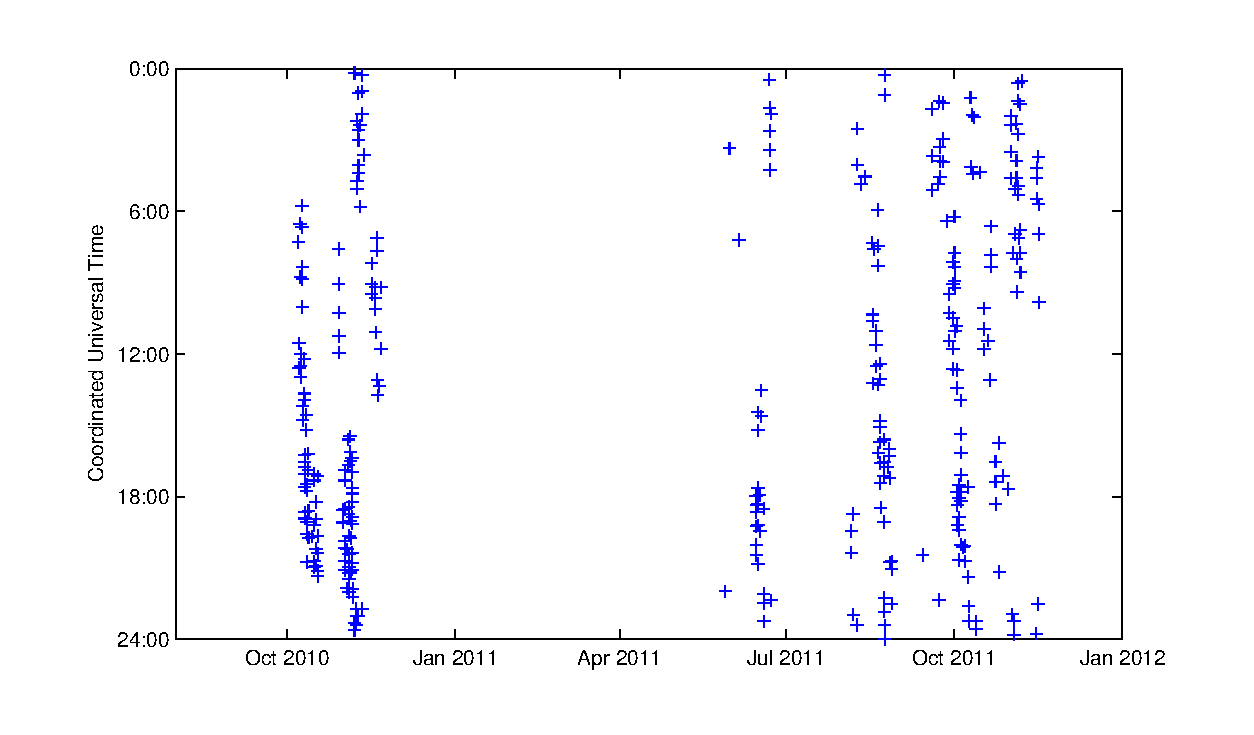
\includegraphics[scale=0.6]{eventTime_date_experiment.eps}
  \caption{The hour when antihydrogen events detected over the period of time during which ALPHA was running in Coordinated Universal Time.}
  \label{fig:eventTime_date_experiment}
\end{figure}


\section{Methods Summary}
A bound on the temporal variation of the antihydrogen charge is performed by comparison of a test statistic $S$, constructed to approximate the magnitude of a Fourier coefficient, of the collected data to simulated distributions of this statistic.  A statistically significant nonzero value of $S$ would indicate a violation of Lorentz Invariance.

The full data set consists of the annihilation times and $z$-values (position along trap axis) from ALPHA's trapping attempts.  Define $f(t)$ to be a function that maps times of $\bar{H}$ annihilations to the $z$ position of those annihilations.  To be continued \ldots

\begin{figure}
  \centering
  \subfigure[\ Full Domain of CDF]{
  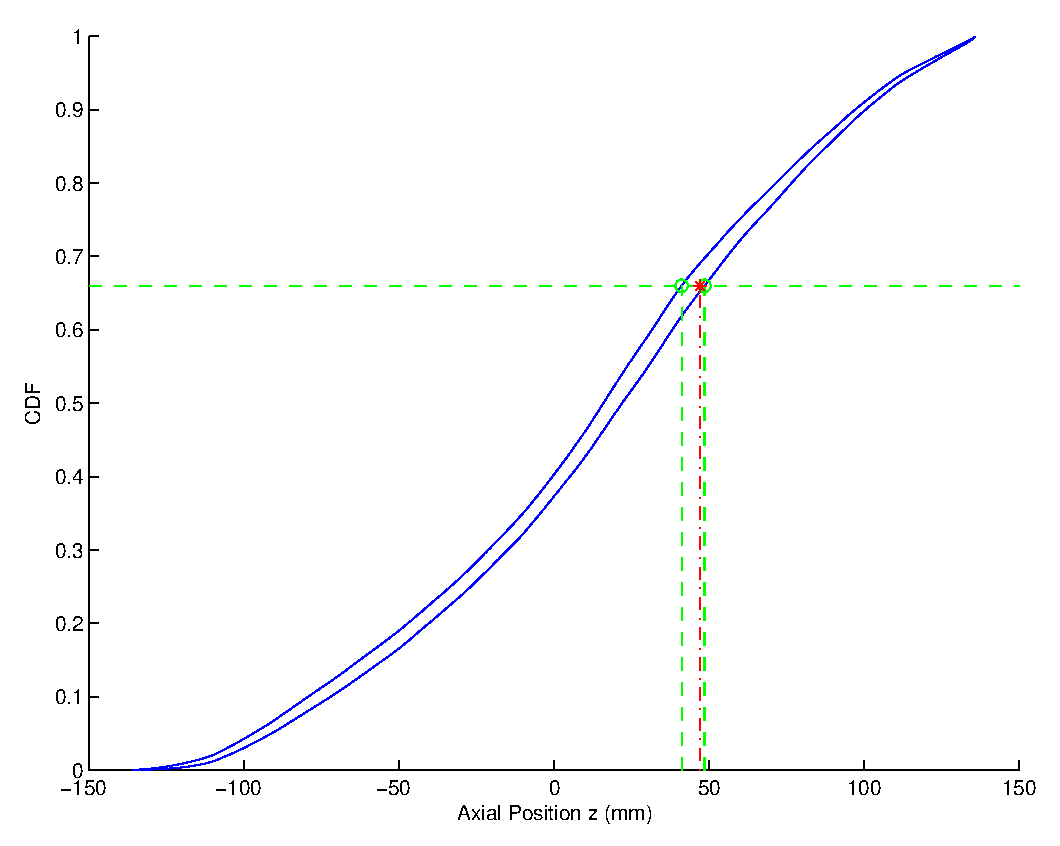
\includegraphics[scale=0.3]{CDF_Interpolation_Plot1.eps}}
  \subfigure[\ Region of Interest]{
  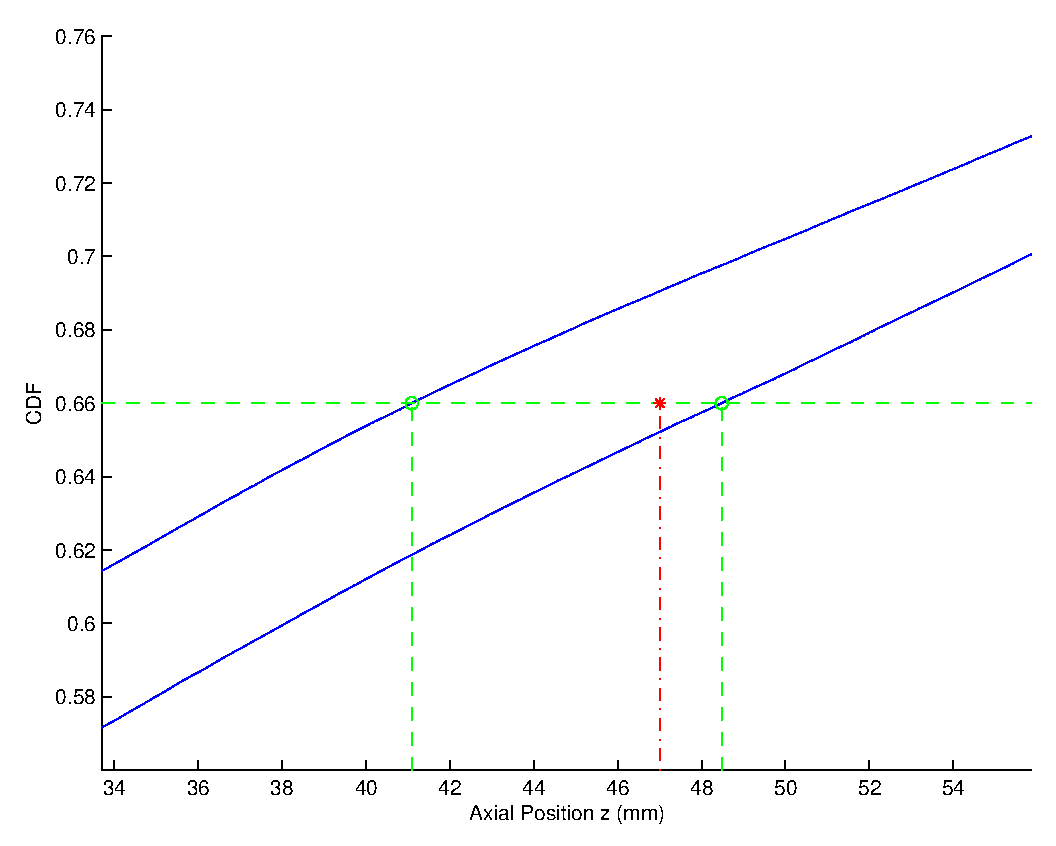
\includegraphics[scale=0.3]{CDF_Interpolation_Plot2.eps}}
  \caption{Graphical depiction of the annihilation $z$ value selection algorithm.  An empirical CDF is generated for several different charges.  Two of such CDFs are shown with linear interpolation (blue solid curves).  When a $z$ position is desired for a given charge, a random value, here shown as 0.66, is picked and the values of the inverse CDFs, which can be read off of the $x$-axis here, are determined (green dashed lines).  The weighted average is then taken to give the $z$ value for the desired charge (red dash-dot line).  Here the charge is closer in value to the charge giving the right CDF than the left CDF.}
  \label{fig:z_interpolation}
\end{figure}

\subsection*{Time Selection}
 The time of antihydrogen annihilation events where sampled in accordance with estimations of $\sim 1900$  trial runs which data was collected in 2010 and 2011 to simulate the time of those 386 events which charge was eligible to be detected.
 
 Here we define a run as a operation for one antihydrogen(s) trapping trial. Dozens of runs were conducted within 128 of 4 $\sim$ 17 hours time schedules when ALPHA were able to access the Antiproton Decelerator and actually tried to trap antyhidrogens. Since we have clock time information of the time of annihilation events in order of a second, mili second of time difference between more than one antyhidrogen annihilations  in a run were ignored.
 
 Within the 128 time spans, the beginning and the time length of the period we can start running the operation, a standby time period, was predicted, since it usually takes time until we become ready for running apparatus after the given AD schedule has been started. The beginning of the time was estimated by Poisson process, which parameter $\lambda$ was 9.3289 /day  with +8.36 minutes shifted, and the time length was estimated by gaussian distribution where the average being 0.2320+-0.1241 day. The annihilation events can only occur within this time period. 
 
 Then the number of runs succeeded in trapping antihydrogen(s) in the standby time span, and the number of the trapped antihydrogens for each run were predicted using Poisson process. Poisson parameters were estimated from the fact that the 386 successful events were observed in 320 runs within 29.6966 days of the total standby time span in the two years of experiment. 
The starting time of the decided number of  successful runs was allocated within the standby time span randomly. The annihilation event time was finally decided by adding 10 minutes of deliberately decided operation time until annihilation happens, to the starting time of the run. The example of times selected with this method is shown in Fig.\ref{fig:eventTime_date_sim}.
 
\begin{figure}
  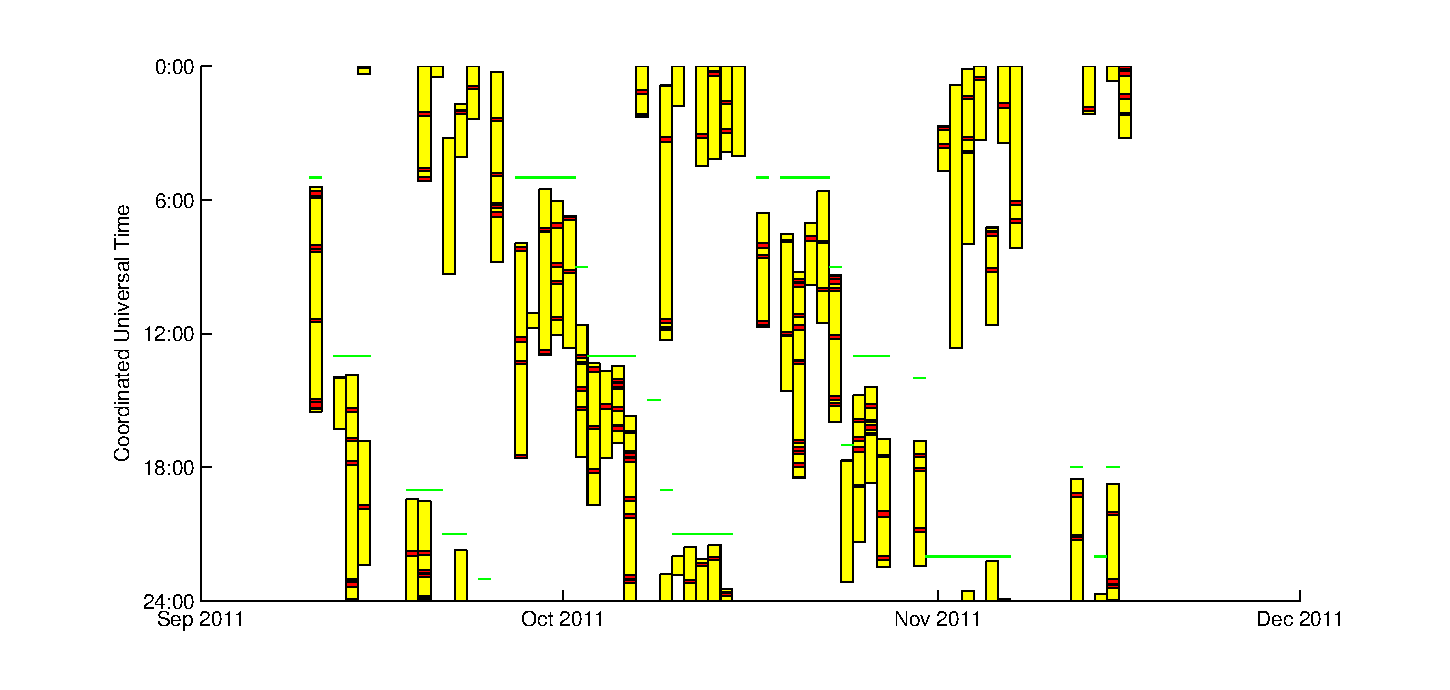
\includegraphics[scale=0.6]{eventTime_sim_example.eps}
  \caption{Time table for one example of time selection in Coordinated Universal Time. The time span when the experiment for trapping antihydrogen are ready to be started (yellow boxes) was chosen regarding to the actual time period when we became able to access to AD (green lines) . Then the number of runs succeeded in trapping antihydrogen, and the starting time  of the run as well as the duration time (red boxes) was chosen. At the time the bottom of red box shows, one to several antihydrogen annihilations annihilates.}
  \label{fig:eventTime_date_sim}
\end{figure}



\subsection*{Position Selection}
Creation of pseudo-data sets requires an algorithm capable of generating $z$ positions of $\bar{H}$ annihilations for arbitrary charge values.  This is achieved by randomly sampling an approximated inverse CDF of the annihilation locations along the trap axis for the given charge.

Using the symplectic integrator discussed in Ref. \onlinecite{amol:14a}, a list of annihilation $z$ coordinates is created for both quip directions for several different charges.  These lists are then adjusted to account for effects from detector smearing and missed detections due to cosmic ray filtering criteria, also discussed in Ref. \onlinecite{amol:14a}.  This provides empirical CDFs of simulated annihilations for various charges.  A simulated $z$ value for these charges can be chosen by selecting a random value from a uniform distribution on the interval (0,1), then determining the associated $z$ value by linearly interpolating the inverse CDF.  For charges between the discrete list of values for which the symplectic integrator has provided results, $z$ positions can be assigned by performing the above interpolation on the two neighboring empirical CDFs using the same random value, then further interpolating by taking a weighted average of the two results.  The weights are chosen to provide a linear interpolation between the two sampled charge distributions.  The process is summarized in Fig. \ref{fig:z_interpolation}.

\begin{acknowledgments}
To be continued\ldots
\end{acknowledgments}

\section{Notes}
The graphs right now are created in Matlab.  In the future they will be made in Origin and should look prettier.

Cite aephem

Look for other papers on charge invariance

Mention this method can be done better in the future

\bibliographystyle{plain}
\bibliography{References.bib,bib.bib}

\end{document}
